\documentclass[12pt,a4paper,titlepage]{article} 
\usepackage[utf8]{inputenc}
\usepackage[spanish]{babel}
\usepackage{graphicx}
\usepackage{booktabs}
\usepackage{geometry}
\usepackage{longtable}
\usepackage{amssymb}
\usepackage{lmodern}
\geometry{a4paper, margin=2.5cm}

\title{\textbf{Planificación Ciclo 2}}
\author{
    \textbf{Grupo 6:} \\
    Guillermo Guhl Arruabarrena \\
    Daniel Gomarín Ruesga \\
    Marcos Romero Villodres \\
    Carlos Sobrino Martin \\
    Javier Pozuelo Ruiz
}
\date{}

\begin{document}

\maketitle

\tableofcontents
\vspace{1cm}

\section{Explicación del Diagrama de Gantt}

El siguiente diagrama de Gantt detalla la planificación y la asignación de las tareas a lo largo del proyecto. La información se corresponde con las estimaciones de esfuerzo total de 65 horas (13 horas por integrante).

\begin{figure}[htbp]
    \centering
    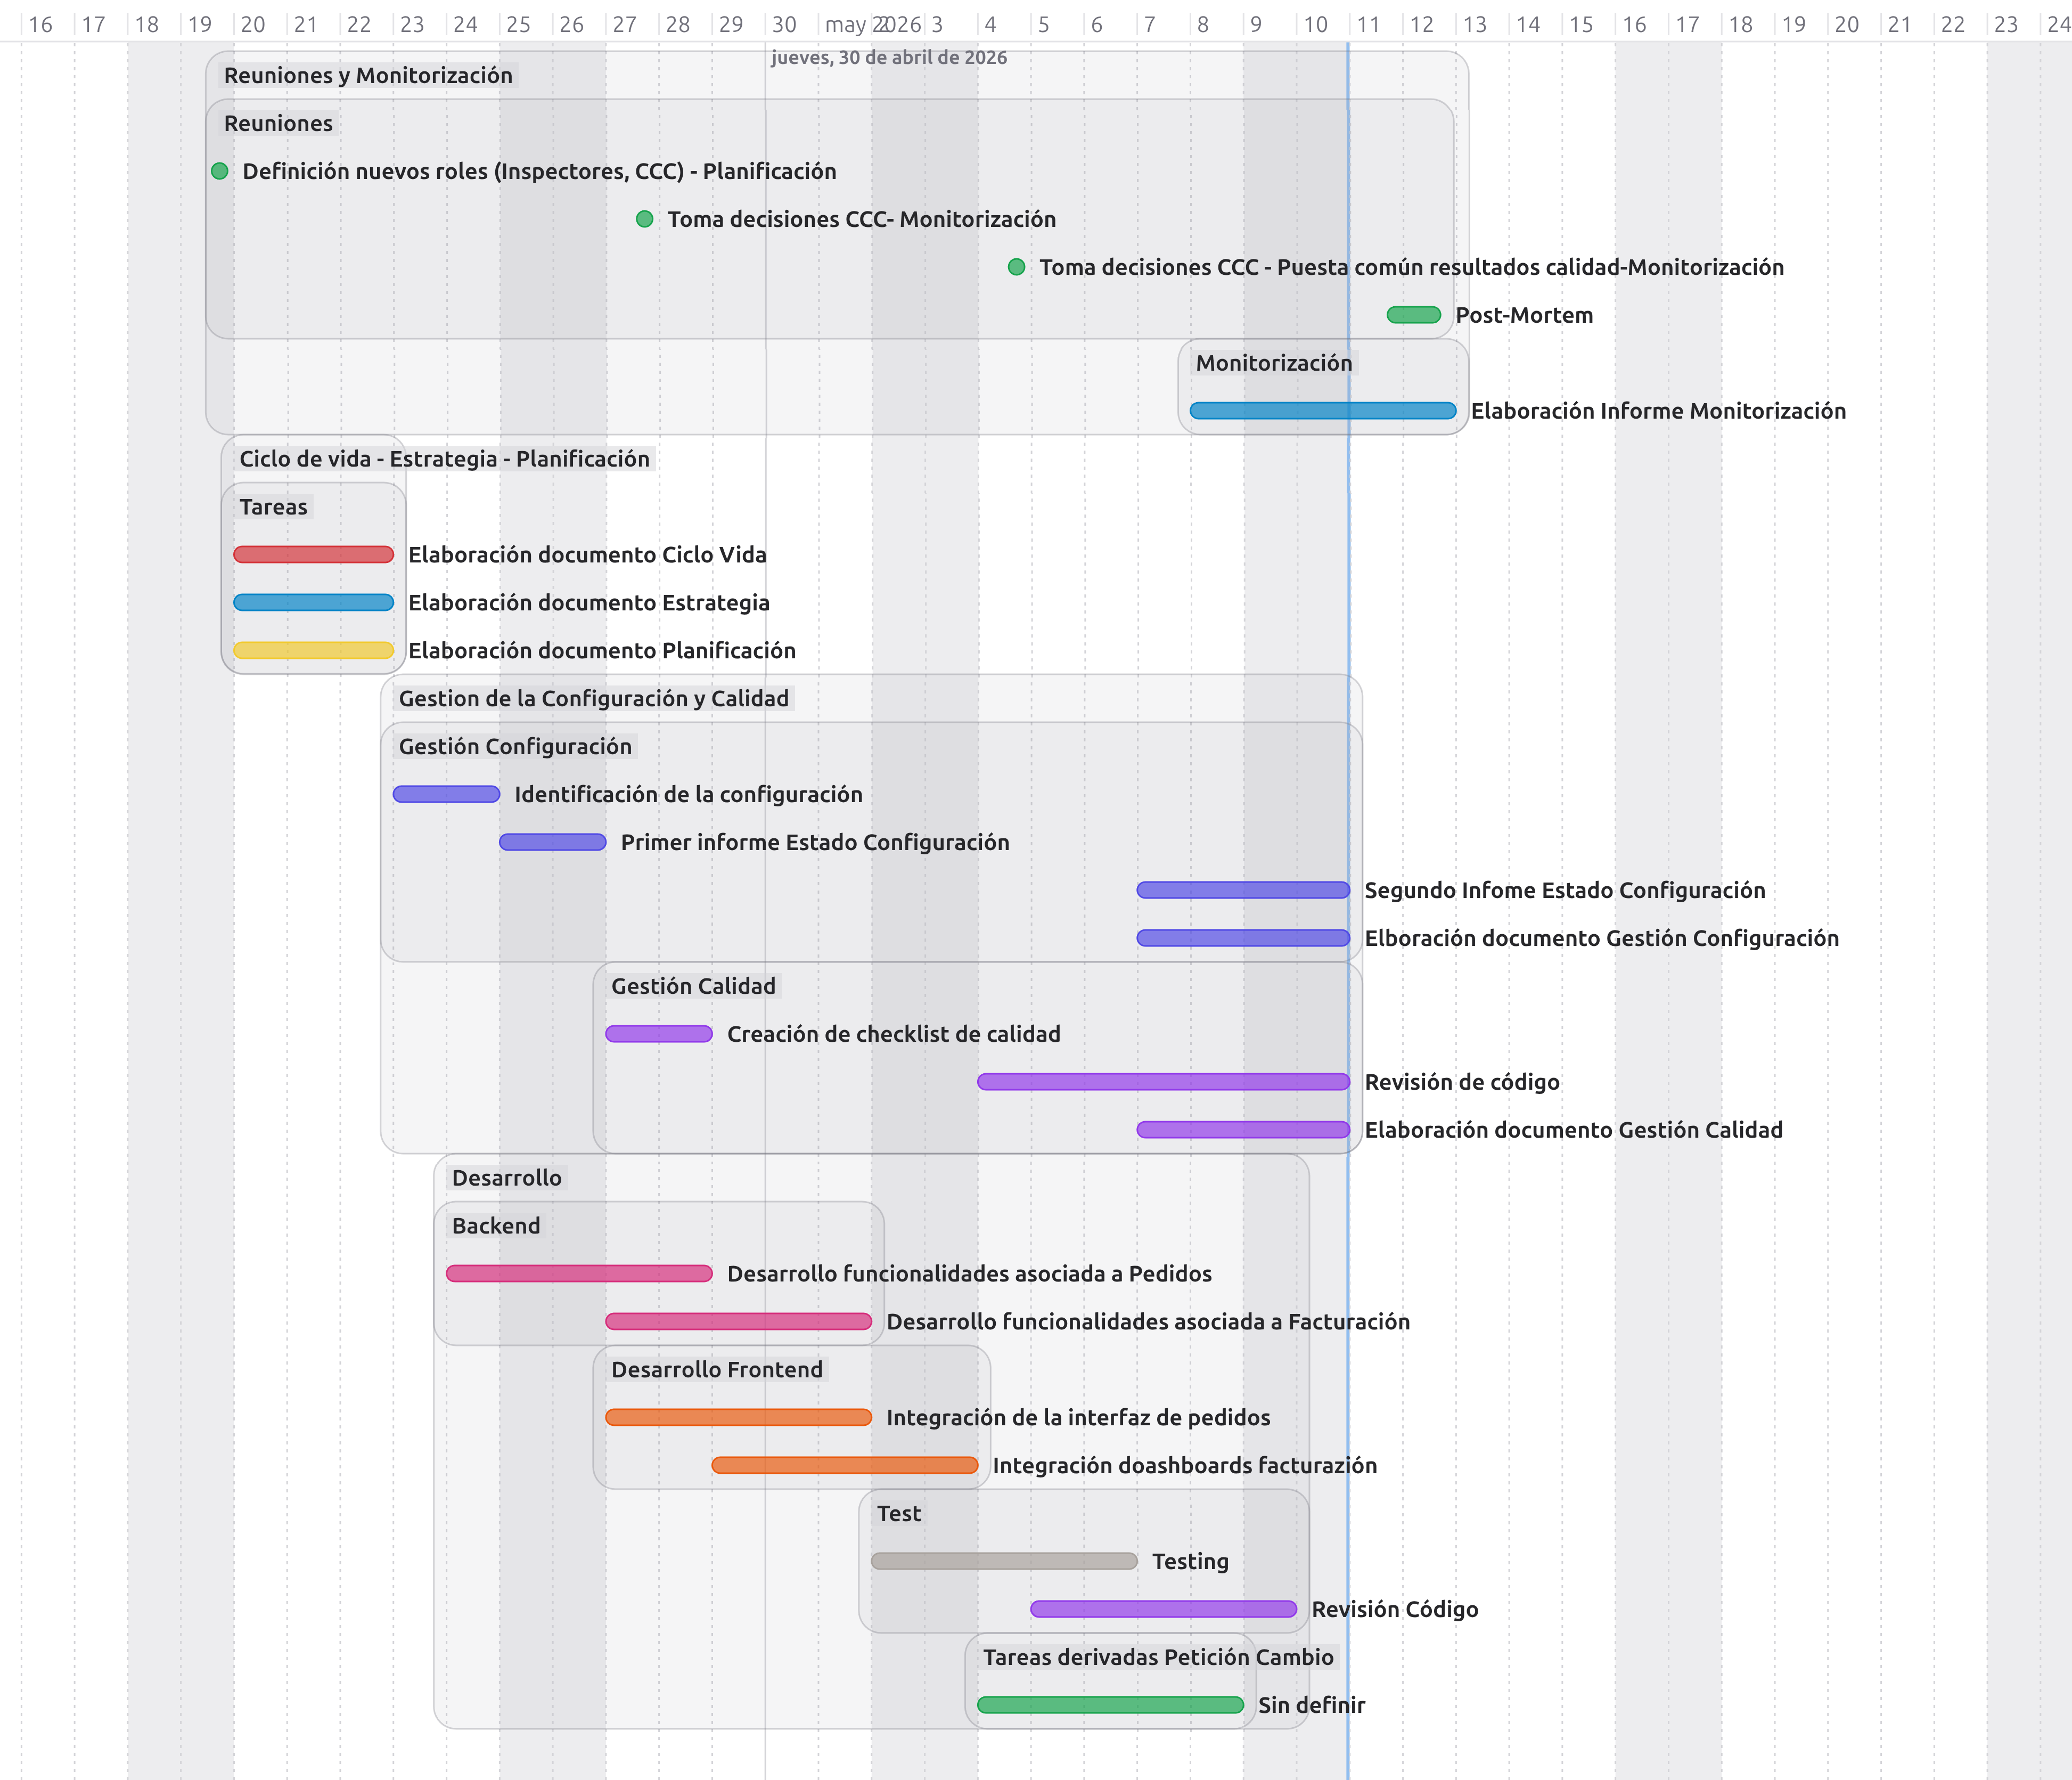
\includegraphics[width=\textwidth]{diagrama_gantt.png} 
    \caption{Diagrama de Gantt de las tareas planificadas.}
    \label{fig:diagrama_gantt}
\end{figure}

A continuación, se detalla el desglose de las tareas respetando la estructura del diagrama:

\begin{itemize}
    \item \textbf{Reuniones y Monitorización} (22h):
    \begin{itemize}
        \item \textbf{Reuniones} (Asignada a: Todos): 15h totales.
        \begin{itemize}
            \item Definición nuevos roles (Inspectores, CCC) - Planificación
            \item Toma decisiones CCC- Monitorización
            \item Toma decisiones CCC - Puesta común resultados calidad-Monitorización
        \end{itemize}
        \item \textbf{Post-Mortem} (Asignada a: Todos): 5h totales.
        \item \textbf{Monitorización}:
        \begin{itemize}
            \item Elaboración Informe Monitorización (Daniel: 2h)
        \end{itemize}
    \end{itemize}

    \item \textbf{Ciclo de vida - Estrategia - Planificación} (3h):
    \begin{itemize}
        \item \textbf{Tareas}:
        \begin{itemize}
            \item Elaboración documento Ciclo Vida (Guillermo: 1h)
            \item Elaboración documento Estrategia (Guillermo: 1h)
            \item Elaboración documento Planificación (Javier: 1h)
        \end{itemize}
    \end{itemize}

    \item \textbf{Gestion de la Configuración y Calidad} (11h):
    \begin{itemize}
        \item \textbf{Gestión Configuración} (Responsable: Marcos):
        \begin{itemize}
            \item Identificación de la configuración (1h)
            \item Primer Informe Estado Configuración (1h)
            \item Segundo Infome Estado Configuración (1h)
            \item Elboración documento Gestión Configuración (1h)
        \end{itemize}
        \item \textbf{Gestión Calidad}:
        \begin{itemize}
            \item Creación de checklist de calidad (Carlos: 2h)
            \item Revisión de código (Guillermo: 3h)
            \item Elaboración documento Gestión Calidad (Carlos: 2h)
        \end{itemize}
    \end{itemize}

    \item \textbf{Desarrollo} (29h):
    \begin{itemize}
        \item \textbf{Backend}:
        \begin{itemize}
            \item Desarrollo Funcionalidades asociada a Pedidos (Javier: 3h)
            \item Desarrollo Funcionalidades asociada a Facturación (Marcos: 2h, Guillermo: 3h)
        \end{itemize}
        \item \textbf{Desarrollo Frontend}:
        \begin{itemize}
            \item Integración de la interfaz de pedidos (Daniel: 3h, Javier: 4h)
            \item Integración doashboards facturación (Daniel: 3h, Marcos: 2h)
        \end{itemize}
        \item \textbf{Test}:
        \begin{itemize}
            \item Testing (Carlos: 2h)
            \item Revisión Código (Carlos: 2h)
        \end{itemize}
        \item \textbf{Tareas derivadas Petición Cambio}:
        \begin{itemize}
            \item Sin definir (Asignada a Todos: 1h por persona, 5h totales)
        \end{itemize}
    \end{itemize}
\end{itemize}

\newpage

\section{Estimación Global de Esfuerzo}

Resumen del esfuerzo total estimado por fase (Total: 65 horas).

\vspace{0.5cm}

\begin{longtable}{@{}lc@{}}
    \toprule
    \textbf{Fase / Grupo} & \textbf{Esfuerzo Estimado} \\ \midrule
    \endfirsthead
    \toprule
    \textbf{Fase / Grupo} & \textbf{Esfuerzo Estimado} \\ \midrule
    \endhead
    \bottomrule
    \endfoot
    \bottomrule

    \textbf{Reuniones y Monitorización} & \textbf{22 h} \\
    $\llcorner$ Reuniones de seguimiento (3) & 15 h \\
    $\llcorner$ Post-Mortem & 5 h \\
    $\llcorner$ Monitorización & 2 h \\ \addlinespace

    \textbf{Ciclo de vida - Estrategia - Planificación} & \textbf{3 h} \\
    $\llcorner$ Tareas de Documentación & 3 h \\ \addlinespace

    \textbf{Gestion de la Configuración y Calidad} & \textbf{11 h} \\
    $\llcorner$ Gestión Configuración & 4 h \\
    $\llcorner$ Gestión Calidad & 7 h \\ \addlinespace

    \textbf{Desarrollo} & \textbf{29 h} \\
    $\llcorner$ Backend & 8 h \\
    $\llcorner$ Desarrollo Frontend & 12 h \\
    $\llcorner$ Test & 4 h \\ 
    $\llcorner$ Tareas derivadas Petición Cambio & 5 h \\ \midrule
    
    \textbf{TOTAL DEL PROYECTO} & \textbf{65 horas} \\
\end{longtable}

\section{Estimación de Esfuerzo por Persona}

Distribución de tareas por integrante (13h totales por persona).

\vspace{0.5cm}

\begin{longtable}{@{}p{4.5cm} p{7.5cm} c@{}}
    \toprule
    \textbf{Integrante} & \textbf{Tareas} & \textbf{Total} \\ \midrule
    \endfirsthead
    \toprule
    \textbf{Integrante} & \textbf{Tareas} & \textbf{Total} \\ \midrule
    \endhead
    \bottomrule
    \endfoot
    \bottomrule

    \textbf{Daniel Gomarín} & 
    - Transversales (Reuniones + Post-Mortem + Petición): 5h \newline
    - Elaboración Informe Monitorización: 2h \newline
    - Integración de la interfaz de pedidos: 3h \newline
    - Integración doashboards facturación: 3h & \textbf{13 h} \\ \midrule

    \textbf{Marcos Romero} & 
    - Transversales (Reuniones + Post-Mortem + Petición): 5h \newline
    - Tareas de Gestión Configuración: 4h \newline
    - Desarrollo Funcionalidades asociada a Facturación: 2h \newline
    - Integración doashboards facturación: 2h & \textbf{13 h} \\ \midrule

    \textbf{Javier Pozuelo} & 
    - Transversales (Reuniones + Post-Mortem + Petición): 5h \newline
    - Elaboración documento Planificación: 1h \newline
    - Desarrollo Funcionalidades asociada a Pedidos: 3h \newline
    - Integración de la interfaz de pedidos: 4h & \textbf{13 h} \\ \midrule

    \textbf{Guillermo Guhl} & 
    - Transversales (Reuniones + Post-Mortem + Petición): 5h \newline
    - Elaboración documento Ciclo Vida: 1h \newline
    - Elaboración documento Estrategia: 1h \newline
    - Revisión de código (Gestión Calidad): 3h \newline
    - Desarrollo Funcionalidades asociada a Facturación: 3h & \textbf{13 h} \\ \midrule

    \textbf{Carlos Sobrino} & 
    - Transversales (Reuniones + Post-Mortem + Petición): 5h \newline
    - Creación de checklist de calidad: 2h \newline
    - Elaboración documento Gestión Calidad: 2h \newline
    - Testing: 2h \newline
    - Revisión Código (Test): 2h & \textbf{13 h} \\ \midrule

    \multicolumn{2}{r}{\textbf{ESFUERZO GLOBAL DEL PROYECTO}} & \textbf{65 h} \\ 
\end{longtable}

\end{document}
